\section{Background}

%%%%%%%%%%%%%%%%%%%%%%%%%%%%%%%%%%%%%%%%%%%%%%%%%%%%%%%%%%%%%%%%%%%%%%%%%%%%%%
\subsection{Cooperativity}

\begin{slide}
    What is Process Cooperativity?
    \begin{figure}
        \subfigure{
            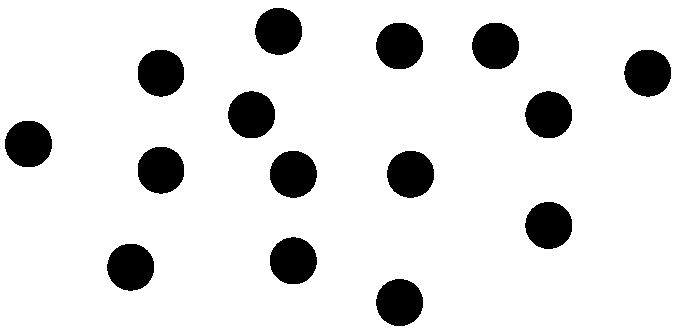
\includegraphics[scale=0.4]{ChugMachine.pdf}
        }
        \hspace{10mm}
        \subfigure{
            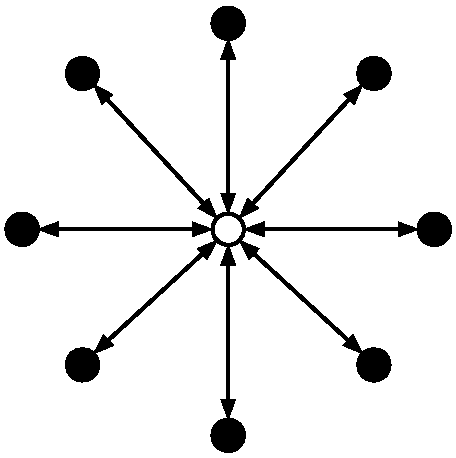
\includegraphics[scale=0.5]{SingleCluster.pdf}
        }
    \end{figure}

    \inote{
        \item Where white represents a channel and black represents a process.
        \item Channel = Source of synchronization (\ie~locks, abstractions, \etc)
        \item[] ~
        \item Left: Cloud of processes with no interaction.
        \item Right: Some sort of batch job? A bit of shared state amongst all processes
                these processes could all really be parallel or be competing, but in 
                either case they cooperate.
        \item DEGREE OF COOPERATIVITY: 
            \begin{itemize}
                \item {\em of process:} flux of interaction with inter-proc comm method.
                \item {\em of system:} rate of interaction between Ps and Cs as both flux in size.
            \end{itemize}
    }
\end{slide}


\begin{slide}
    What does Cooperativity give us?
    \begin{figure} 
    \centering
        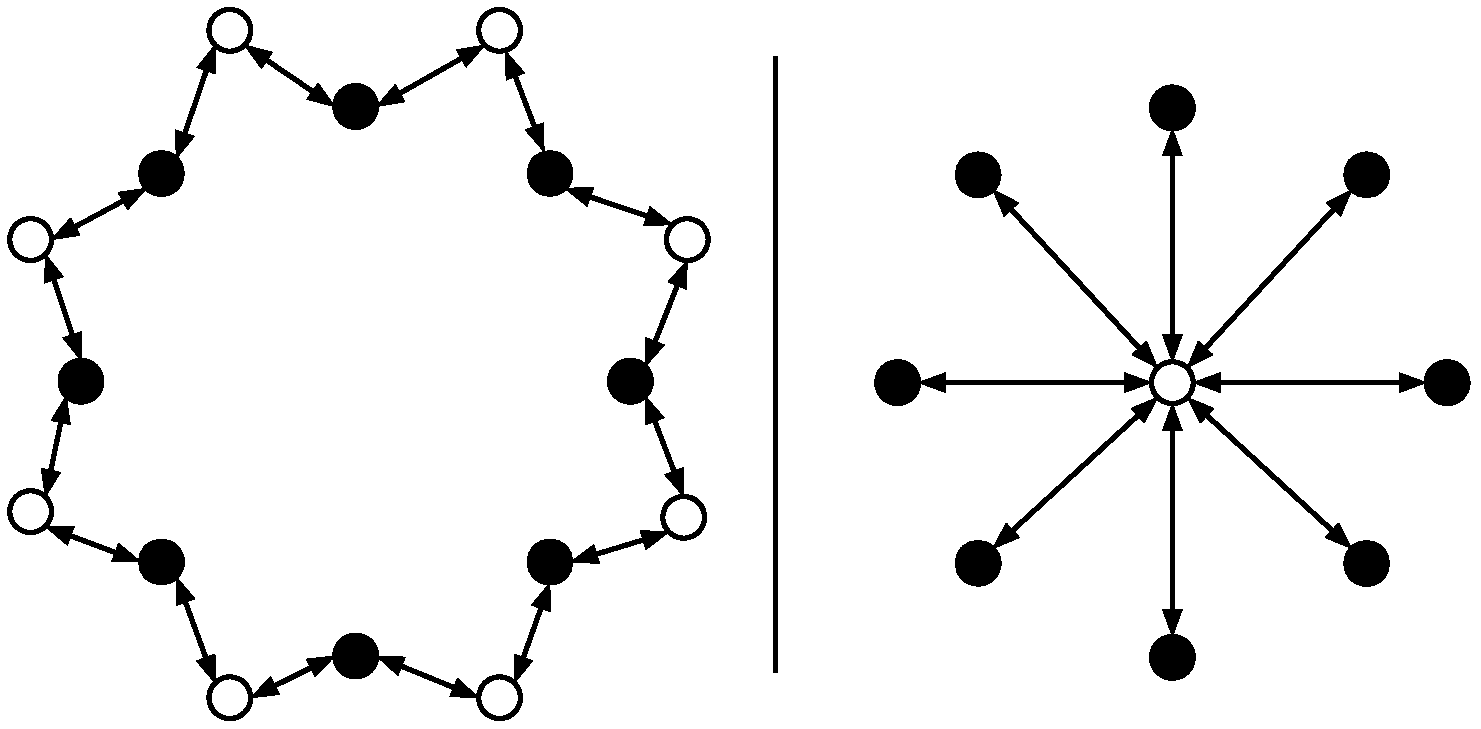
\includegraphics[scale=0.4]{RingVCluster.pdf}
        \label{fig:RingVCluster}
    \end{figure}

    \note{
        Whats the difference in cooperativity in the left and right
        set of processes?         \begin{itemize}
            \item Left: A Ring, the level of parallelism is nearly nil. Each
                process is cooperating yes, but the granularity of the 
                application is very fine.

            \item Right: A Star, the level of parallelism is nearly full. Each
                process is cooperating, and is {\bf not reliant on more than one} 
                other.
        \end{itemize}
        Overall, what can be gained by looking at cooperativity in terms of
        understanding the applications behaviour? Knowing the granularity of
        parallelism.\\
        ~\\
        \hfill
        Next: what is a minimal inter-proc comm method?
    }
\end{slide}


%%%%%%%%%%%%%%%%%%%%%%%%%%%%%%%%%%%%%%%%%%%%%%%%%%%%%%%%%%%%%%%%%%%%%%%%%%%%%%
\subsection{Message Passing}

\begin{slide}
    We use a Symmetric, Synchronous, Message-Passing Primitive: 
            \begin{center} {\tt\large swap} \end{center}
    \begin{itemize}
        \item Purely captures cooperation of processes by synchronizing on
                the shared channel.
        \item Ultimately can be extended to take into account:
            \begin{itemize}
                \item Directionality
                \item Asynchrony
            \end{itemize}
    \end{itemize}
    \inote{
       \item Async: while user code doesn't block, there is blocking
             in terms of the channel implementation. This is not
             indicated (in most cases) to the scheduler.
       \item Sync: The issue of process cooperation has been elevated
             to the process level for the scheduler to directly involve
             itself.
       \item
        Ultimately there is nothing stopping us from choosing the other
        types of message passing, but it would conflate the issue of
        process cooperativity if all we are after is whether two processes
        are cooperating on some task.\\
        ~\\
        \hfill
        Next: How would we use coop as a feedback metric?\\ 
        \hfill
        What does that mean?
    }
\end{slide}


%%%%%%%%%%%%%%%%%%%%%%%%%%%%%%%%%%%%%%%%%%%%%%%%%%%%%%%%%%%%%%%%%%%%%%%%%%%%%%
\subsection{Runtime Scheduling}

\begin{slide}
    \begin{itemize}
        \item Schedulers can be defined in a discrete manner:
            \begin{enumerate}
                \item {\em Choose} a process from set
                \item {\em Reduce} it
                \item {\em Update} private scheduler state
            \end{enumerate}
        \item Statistics can be gathered at every step about process:
            \begin{itemize}
                \item Number of channel partners,
                \item Timestamp of last run,
                \item Number of reductions, \etc
            \end{itemize}
        \item {\sl What statistics are neccessary for recognizing cooperativity?}
    \end{itemize}

    \inote{
        \item Choosing from set: Top Always (batching), Queue (Round-Robin)
        \item Reductions Return some indication: yield/blocked, unblocked, completed, nothing
        \item Update state based on historical data.
            \begin{itemize}
                \item Timestamp of last run = Separate between batching/round-robin
                \item Cooperativity metrics: yields, partners, thus longevity and granularity 
            \end{itemize}
        \item gets back to why we chose swap:
            \begin{itemize}
                \item (if asymmetrical, we would have a harder time with 'partner')
                \item (if async, we would have a harder time with 'yield' and noticing longevity/progress)
            \end{itemize}
    }
\end{slide}

